\subsection{Serializability}

\label{sec:ser}

The operational semantics for \tpl\ defined in Section \ref{sec:2plSemantics} claim that, given the adherence to the two phase protocol, they guarantee the serializability of the histories of operations that arise from program executions. This section is dedicated to proving such statement by analyzing traces produced by programs. We begin with some preliminary definitions followed by auxiliary lemmata and finally a formal proof of serializability.

\tocless\subsubsection{Traces}

Since serializability is a property of program histories our proof will use them and we therefore here introduce and formalize the concept of a trace.

\begin{defn}
	(Trace).
	A \emph{trace} is an ordered sequence of operations that are generated by the reduction of a generic program under the \tpl\ semantics. It comes from the set $[\mathsf{Act} \times \mathds{N}]$ which is ranged over by $\tau, \tau_1, \ldots, \tau_n$. Every element of a trace is a tuple with an action label and an ordinal number to represent the numerical index of the operation.
\end{defn}

We refer to elements of a trace as operations, often using $op, x, y$ to range over them. We only study the particular kind of traces that arises from a program which succesfully terminates and reduces to $\pskip$. Such traces can be retrieved from program executions using the $\mathsf{trace}$ function, that given a storage, transactions stack and program, returns one of the possible traces that are produced by the operational semantics starting with the input state.
\begin{align*}
	\pred{trace}{h, \Phi, S, \mathds{P}} &\triangleq \pred{trace'}{h, \Phi, S, \mathds{P}, 0} \\
	\pred{trace'}{h, \emptyset, S, \pskip, n} &\triangleq [] \\
	\pred{trace'}{h, \Phi, S, \mathds{P}, n} &\triangleq (\alpha, n) : \pred{trace'}{h', \Phi', S', \mathds{P}', n+ 1}
	\\
	\text{where }& (h, \Phi, S, \mathds{P}) \xrightarrow{\alpha} (h', \Phi', S', \mathds{P}') \rightarrow^* (h'', \emptyset, S'', \pskip)
\end{align*}

To better illustrate concrete traces we provide an example program with its corresponding formally generated trace. Consider the program and trace in Figure \ref{fig:2pltrace}. The first transaction assigns $5$ value to variable $\pvar{x}$ and later mutates the same cell to write value $2$. The other one checks whether cell indexed with $5$ has a value of $2$ and if so, it updates it back to $0$. In the execution preliminaries, the two user transactions get converted into system one and are assigned with identifiers, $4$ and $1$ respectively. Later, transaction $4$ acquires the lock on $5$ in exclusive mode, meaning it will complete the reduction of its commands before $1$ starts with its own ones. since it needs the same lock in shared mode first, then in the exclusive one to complete the update.

\begin{figure}
\[
	\begin{array}{l r}
		\begin{array}{l || l}
			\begin{array}{l}
				\mathtt{begin} \\
					\quad \passign{\pvar{x}}{5} ; \\
					\quad \pmutate{\pvar{x}}{2} \\
				\mathtt{end}
			\end{array}
				&
			\begin{array}{l}
				\mathtt{begin} \\
					\quad \pderef{\pvar{y}}{5} ; \\
					\quad \pifs{\pvar{y} = 2} \\
					\quad \quad \pmutate{5}{0} \\
					\quad \pifm \\
					\quad \quad \pskip \\
				\mathtt{end}
			\end{array}
		\end{array}
		&
		\begin{array}{r l}
			\tau =
			&
			\left[
			\begin{aligned}
				&(\actid{1}, 0), (\actid{4}, 1), (\actid{4}, 2), (\actlock{4}{5}{\textsc{x}}, 3), \\
				&(\actid{4}, 4), (\actwrite{4}{5}{2}, 5), (\actunlock{4}{5}, 6), \\
				&(\actlock{1}{5}{\textsc{s}}, 7), (\actid{4}, 8), (\actread{1}{5}{2}, 9), \\
				&(\actid{4}, 10), (\actid{4}, 11), (\actlock{1}{5}{\textsc{x}}, 12), \\
				&(\actwrite{1}{5}{0}, 13),  (\actunlock{1}{5}, 14), \\
				&(\actid{4}, 15), (\actprog, 16)
			\end{aligned}
			\right]
		\end{array}
	\end{array}
\]
\captionof{figure}{A program with parallel composition of two transaction and a possible trace generated by the execution under \tpl\ semantics.}
\label{fig:2pltrace}
\end{figure}

Going back to formal definitions, we say that an operation $op \in \mathsf{Act} \times \mathds{N}$ belongs to a trace $\tau$, written $op \in \tau$ if and only if $op \in \tau = \top$ where the $\in$ predicate is defined as follows:
\begin{align*}
	(\alpha, n) \in [] &\overset{\text{def}}{\iff} \bot \\
	(\alpha, n) \in (\alpha, n):\tau &\overset{\text{def}}{\iff} \top \\
	(\alpha, n) \in (\alpha', n'):\tau &\overset{\text{def}}{\iff} (\alpha, n) \in \tau
\end{align*}

For conciseness, we often overload the $\in$ function to cope with actions only, without the numerical component, and write $\alpha \in \tau$ to actually mean $\exists n \ldotp (\alpha, n) \in \tau$. It is often useful to express the order of operations as part of a trace. For this reason, we introduce the precedence of operations which asserts that two operations belong to the trace and their respective indexes are correctly ordered.
\begin{defn}
	(Operation precedence).
	The \emph{operation precedence} as part of a trace $\tau$, written $\tau \vDash x < y$, is defined in the following way:
	\[
		\tau \vDash (\alpha, n) < (\alpha', n') \overset{\text{def}}{\iff}
(\alpha, n) \in \tau \land (\alpha', n') \in \tau \land n < n'
	\]
\end{defn}

For conciseness, we overload the definition of $<$ to cope with the ordering of a concrete operation and a generic action (i.e. the first component of an operation) and of two generic actions without an associated index.
\begin{align*}
	\tau \vDash op < \alpha \overset{\text{def}}{\iff}&
	\exists n \ldotp \tau \vDash op < (\alpha, n)
		\\
	\tau \vDash \alpha < op \overset{\text{def}}{\iff}&
	\exists n \ldotp \tau \vDash (\alpha, n) < op
		\\
	\tau \vDash \alpha < \alpha' \overset{\text{def}}{\iff}&
	\exists n, n' \ldotp \tau \vDash (\alpha, n) < (\alpha', n')
\end{align*}

This allows to assert on the existence of some particular action appearing before or after another one as part of a trace which will prove very useful in proofs. Two different actions which are part of the same trace are in conflict if they are performed by different transactions and one of them is a write or alloc while the other one is a read, write or alloc on the same key. These are treated specially since the order in which they appear might affect the end result of the program execution.

\begin{defn}
	\label{defn:conflict}
	(Conflicting actions).
	Actions $\alpha$ and $\alpha'$ are \emph{conflicting} if and only if they both belong to the same trace $\tau$ and $\pred{conflict}{\alpha, \alpha'} = \top$, where the $\mathsf{conflict}$ predicate is defined as:
	\begin{align*}
		\pred{conflict}{\actwrite{i}{k}{v}, \actwrite{j}{k}{v'}} &\overset{\text{def}}{\iff} i \neq j
			\\
		\pred{conflict}{\actwrite{i}{k}{v}, \actread{j}{k}{v'}} &\overset{\text{def}}{\iff} i \neq j
			\\
		\pred{conflict}{\actread{i}{k}{v}, \actwrite{j}{k}{v'}} &\overset{\text{def}}{\iff} i \neq j
			\\
		\pred{conflict}{\actalloc{i}{n}{l}, \actread{j}{k}{v'}} &\overset{\text{def}}{\iff} i \neq j \land l \leq k < l + n
			\\
		\pred{conflict}{\actalloc{i}{n}{l}, \actwrite{j}{k}{v'}} &\overset{\text{def}}{\iff} i \neq j \land l \leq k < l + n
			\\
		\pred{conflict}{\alpha, \alpha'} &\overset{\text{def}}{\iff} \bot
	\end{align*}
\end{defn}
We overload Definition \ref{defn:conflict} to also cope with trace operations, by simply unwrapping them and extracting the corresponding action part of the tuple.
\[
	\pred{conflict}{(\alpha, n), (\alpha', n')} \triangleq \pred{conflict}{\alpha, \alpha'}
\]

Finally, in order to aid the clarity of property definitions regarding traces, we define two predicates describing particular operations. The first one, $op(\iota)$, refers to any action performed by transaction $\mathds{T}_\iota$.
\begin{align*}
	op(\iota) \triangleq (\alpha, n) \text{ s.t. } \alpha \in \{ &\actid{\iota}, \actwrite{\iota}{k}{v}, \actlock{\iota}{k}{\kappa}, \actunlock{\iota}{k}, \actread{\iota}{k}{v},
	\\
	&\actalloc{\iota}{m}{l}\ |\ k, l \in \mathsf{Key}, v \in \mathsf{Val}, n \in \mathds{N}, \kappa \in \mathsf{Lock}, m \in \mathds{N} \} \land n \in \mathds{N} \}
\end{align*}
Similarly, the $op(\iota, k)$ predicate describes any operation done by the transaction identified with $\iota$, which accesses item $k$, i.e. either reading, writing or allocating it.
\begin{align*}
	op(\iota, k) \triangleq (\alpha, n) \text{ s.t. } \alpha \in\ &\{ \actread{\iota}{k}{v}, \actwrite{\iota}{k}{v}\ |\ v \in \mathsf{Val} \}\
	\cup \\
	&\{\actalloc{\iota}{m}{l}\ |\ m \in \mathds{N}, l \in \mathsf{Key}, l \leq k < l + m \} \land n \in \mathds{N}
\end{align*}

The two following definitions empower us to formally define the serializability of traces. We start by describing what it means for a trace $\tau$ to be serial: intuitively, $\tau$ is the result of running a program where transactions are executed in a sequential fashion, with no interleaving of operations. Next, we define the concept of equivalence between traces. This is expressed by imposing the equality on their operations and transactions, but not strictly on the order in which they appear. In fact, only conflicting operations are required to be ordered in the same way.

\begin{defn}
	(Trace equivalence).
	Two traces $\tau, \tau' \in [\mathsf{Act} \times \mathds{N}]$ are defined to be \emph{equivalent}, written $\tau \equiv \tau'$, if and only if they contain the same transactions and operations and if they order conflicting operations in the same way.
	\begin{gather*}
		\tau \equiv \tau' \iff \\
		(\forall \iota, x \ldotp x = op(\iota) \lor x = \actprog \implies (x \in \tau \iff x \in \tau'))\ \land \\
		(\forall x, x', i, j, k \ldotp x = op(i, k) \land x' = op(j, k) \land \pred{conflict}{x, x'}
		\implies (\tau \vDash x < x' \iff \tau' \vDash x < x'))
	\end{gather*}
\end{defn}

\begin{defn}
	(Serial trace).
	A trace $\tau$ is defined as \emph{serial} if and only if for any two transactions, $i$ and $j$, inside of it either all of $i$'s operations appear before $j$'s ones or all of $j$'s operations appear before $i$'s ones.
	\begin{gather*}
		\pred{serial}{\tau} \iff \\
		\forall i, j \ldotp i \neq j \land op(i) \in \tau \land op(j) \in \tau \implies \\
		(\forall x, x' \ldotp x = op(i) \in \tau \land x' = op(j) \in \tau \implies \tau \vDash x < x') \\
		\lor \\
		(\forall x, x' \ldotp x = op(i) \in \tau \land x' = op(j) \in \tau \implies \tau \vDash x' < x)
	\end{gather*}
\end{defn}

\begin{defn}
	(Serializable).
	A trace $\tau$ is \emph{serializable} if and only if it is equivalent to some serial trace $\tau'$.
	\[
		\pred{serializable}{\tau} \iff \exists \tau' \ldotp \pred{serial}{\tau'} \land \tau \equiv \tau'
	\]
\end{defn}

\begin{center}
	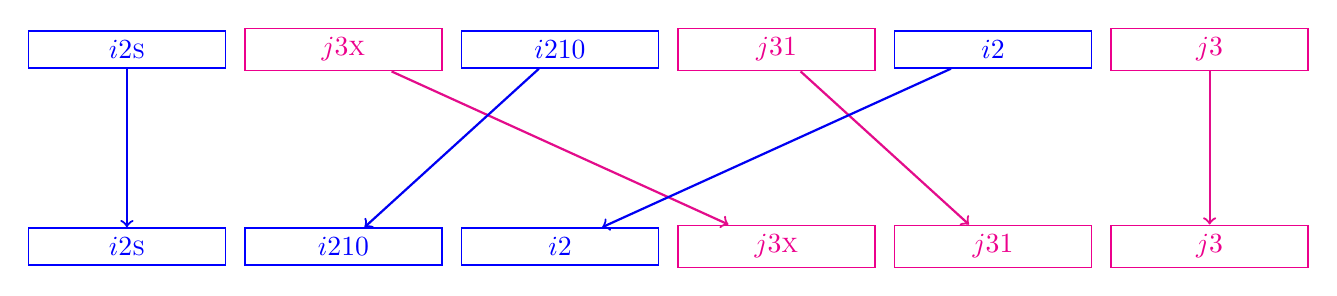
\begin{tikzpicture}[->, semithick]
		\tikzset{
		    tleft/.style= {rectangle, draw=blue, color=blue, minimum width=2.5cm},
		    tright/.style= {rectangle, draw=magenta, color=magenta, minimum width=2.5cm},
		    pleft/.style= {above, black!5!blue, thick},
		    pright/.style= {above, black!5!magenta, thick},
		}
		
		\node[tleft] (s1) at (0, 0) {$\actlock{i}{2}{\textsc{s}}$};
		\node[tright] (s2) at (2.75, 0) {$\actlock{j}{3}{\textsc{x}}$};
		\node[tleft] (s3) at (5.5, 0) {$\actread{i}{2}{10}$};
		\node[tright] (s4) at (8.25, 0) {$\actwrite{j}{3}{1}$};
		\node[tleft] (s5) at (11, 0) {$\actunlock{i}{2}$};
		\node[tright] (s6) at (13.75, 0) {$\actunlock{j}{3}$};
		
		\node[tleft] (s7) at (0,-2.5) {$\actlock{i}{2}{\textsc{s}}$};
		\node[tleft] (s8) at (2.75,-2.5) {$\actread{i}{2}{10}$};
		\node[tleft] (s9) at (5.5,-2.5) {$\actunlock{i}{2}$};
		\node[tright] (s10) at (8.25,-2.5) {$\actlock{j}{3}{\textsc{x}}$};
		\node[tright] (s11) at (11,-2.5) {$\actwrite{j}{3}{1}$};
		\node[tright] (s12) at (13.75,-2.5) {$\actunlock{j}{3}$};
		
		\draw
		(s1) edge[pleft] (s7)
		(s2) edge[pright] (s10)
		(s3) edge[pleft] (s8)
		(s4) edge[pright] (s11)
		(s5) edge[pleft] (s9)
		(s6) edge[pright] (s12);
	\end{tikzpicture}
	\captionof{figure}{A serializable trace at the top with one of the corresponding equivalent and serial traces.}
\end{center}

\tocless\subsubsection{Graphs}

\label{sec:graphs}

The proof of serializability will be carried over a particular representation of traces that we introduce in this section. We utilize serialization graphs in order to describe relationships between transactions participating in a program execution.

\begin{defn}
	\label{defn:sg}
	(Serialization graph).
	The \emph{serialization graph} of a given trace $\tau$ is a directed graph whose nodes are the identifiers of all the transactions that perform an action as part of $\tau$ and whose edges are between transactions that have ordered conflicting operations according to $\tau$.
	\begin{align*}
		\pred{SG}{\tau} &\triangleq (N, E) \\[0.4em]
		\text{where } N &\triangleq \{ \iota\ |\ op(\iota) \in \tau \} \\[0.4em]
		E &\triangleq
			\left\{
				\begin{array}{r | l}
					(i, j)
					&
					\begin{array}{c}
						x = op(i, k) \land x' = op(j, k) \\
						\land\ \pred{conflict}{x, x'}
						\land \tau \vDash x < x' 
					\end{array}
				\end{array}
			\right\}
	\end{align*}
\end{defn}

Edge connections and paths within a graph $G = (N, E)$ are described by introducing an arrow notation. We write $i \rightarrow j \in G$ to indicate that there is an edge from node $i$ to node $j$ in $E$. In the following list of statements, we make an abuse of notation to allow more expressive formulas and add a transitive closure arrow ($\rightarrow^*$) that is able to describe a path in the graph.
\[
	\begin{array}{c @{\hspace{30pt}} c}
		\begin{aligned}
			i \rightarrow j \in E &\triangleq (i, j) \in E \\
			i \rightarrow^1 j \in E &\triangleq i \rightarrow j \in E \\
			i \rightarrow^* j \in E &\triangleq \exists n \ldotp i \rightarrow^n j \in E
		\end{aligned}
		&
		\begin{aligned}
			i \rightarrow j \in G &\triangleq i \rightarrow j \in G \downarrow_2 \\
			i \rightarrow^n j \in E &\triangleq \exists t \ldotp i \rightarrow t \in E \land t \rightarrow^{n-1} \in E \\
			i \rightarrow^* j \in G &\triangleq i \rightarrow^* j \in G \downarrow_2
		\end{aligned}
	\end{array}		
\]

Our goal is now to prove that all traces whose serialization graph contains no cyclic paths are serializable. We do this by first formally introducing the acyclic property of graphs and later the concept of a topological order of a graph.

\begin{defn}
	(Acyclic graph).
	A graph $G = (N, E)$ is \emph{acyclic} if and only if there is no path in $G$ that connects a node in $N$ to itself.
	\[
		\pred{acyclic}{G} \iff \forall a \ldotp a \in G \downarrow_1 \implies \lnot a \rightarrow^* a \in G
	\]
\end{defn}

\begin{defn}
	(Topological sort).
	A \emph{topological sort} of a graph $G = (N, E)$ is an ordered sequence of all nodes in $N$ such that if node $a$ appears before node $b$ in the sequence, then there is no path from $b$ to $a$ in $G$.
	\begin{gather*}
		t = \pred{topo}{(N, E)} \iff \\
		(\forall n \ldotp n \in t \iff n \in N) \land (\forall a, b \ldotp t \vDash a < b \implies \lnot b \rightarrow^* a \not\in E)
	\end{gather*}
\end{defn}

The following theorem establishes a key property we later need in order to prove serializability of the operational semantics introduced in Section \ref{sec:2plSemantics}. The process will in fact start by building the serialization graph of an arbitrary trace arising from \tpl\ semantics, showing that under any circumstance it is acyclic and therefore serializable. This fundamental relationship is established in Theorem \ref{thm:acySer} where we obtain the needed result.
\begin{thm}
	\label{thm:acySer}
	(Acyclic means serializable).
	Every trace that has a serialization graph with no cycles is serializable \cite{ccontrol}.
	\[
		\forall \tau \ldotp \pred{acyclic}{\pred{SG}{\tau}} \implies \pred{serializable}{\tau}
	\]
	
	\begin{proof}
	Let's assume that $\tau \in [\mathsf{Act} \times \mathds{N}]$ is a trace which includes operations coming from transactions identified with $N = \{ \iota_1, \ldots, \iota_m \}$ for a finite $m$. It follows that $N$ is also the set of nodes of $\pred{SG}{\tau}$. By our original assumption we know that $\pred{SG}{\tau}$ is acyclic. For this reason we can always find a topological sort $t = \pred{topo}{\pred{SG}{\tau}} = [t_{\iota_1}, \ldots, t_{\iota_m}]$. Let $\tau'$ be the serial trace that includes transactions (in the presented order) identified with $t_{\iota_1}, \ldots, t_{\iota_m}$ and has all of the same operations as $\tau$. Let $x = op(i, k)$ and $x' = op(j, k)$ such that $\pred{conflict}{x, x'}$ holds and $\tau \vDash x < x'$. By definition of serialization graph, $i \rightarrow j \in \pred{SG}{\tau}$. Therefore, in any topological sort of $\pred{SG}{\tau}$, $i$ must appear before $j$. As a consequence, all of $i$'s operations appear before $j$'s ones in $\tau'$ and in particular $\tau' \vDash x < x'$. By construction, $\tau'$ is serial and it contains all of $\tau$'s operations and we showed that any two conflicting operations are ordered in the same way. We can conclude that $\tau \equiv \tau'$ which implies that $\tau$ is serializable.
	\end{proof}
\end{thm}

\tocless\subsubsection{Proof}

The list of lemmata that follows, describes concrete properties on arbitrary traces $\tau$ generated from the \tpl\ operational semantics rules. The proof process follows a similar structure as the one defined in \cite{papa} and \cite{ccontrol}.

We first introduce and prove all the required properties that serve as building blocks for the final proof. The initial step is to determine that all read, write or allocation actions performed by a transaction, are always followed by an unlock action on the same key done by the same transaction.

\begin{lem}
	\label{prop:unlock}
	(Proof in \ref{lem:unlock}).
	\[
		\forall \tau, \iota, k, \kappa, x \ldotp
		x = op(\iota, k) \land x \in \tau \implies \left( \tau \vDash x < \actunlock{\iota}{k} \right)
	\]
\end{lem}

Conversely, we are also required to show that anytime a particular transaction accesses a storage item through a $\mathsf{read}$ or $\mathsf{write}$ operation, it locks the corresponding entry in the lock manager using the required lock mode. Thus, we first show that all reads are preceded by the appropriate shared lock acquisition.
\begin{lem}
	\label{prop:read}
	(Proof in \ref{lem:read}).
	\begin{gather*}
		\forall \tau, \iota, k, v, \kappa, x, n \ldotp \\
		x = (\actread{\iota}{k}{v}, n) \land x \in \tau \implies \left( \tau \vDash \actlock{\iota}{k}{\kappa} < x \land \kappa \geq \textsc{s} \right)
	\end{gather*}
\end{lem}

Then, for the $\mathsf{write}$ case, we also show that all writes to a cell are preceded by the appropriate exclusive lock acquisition.
\begin{lem}
	\label{prop:write}
	(Proof in \ref{lem:write}).
	\begin{gather*}
		\forall \tau, x, i, k, v, n \ldotp
		x = (\actwrite{i}{k}{v}, n) \land x \in \tau \implies
		\tau \vDash \actlock{i}{k}{\textsc{x}} < x
	\end{gather*}
\end{lem}

The lock manager is not only modified with $\mathsf{lock}$ and $\mathsf{unlock}$ operations, but also with the allocation of new storage cells, which enlarges the domain of the storage and locks the new cells into exclusive mode. In relation to this, we prove that a read or write operation accessing a cell allocated as part of the trace, must appear after the corresponding alloc action. On top of this, we also show that the transaction responsible for allocating the cell will always be the first one to release the lock it holds on it, before any other transaction is able to lock it.
\begin{lem}
	\label{prop:allocBefore}
	(Proof in Lemma \ref{lem:allocBefore}).
	\begin{gather*}
		\forall \tau, i, j, x, x', n, n', l, m, k, v, \kappa \ldotp \\
		x = (\actalloc{i}{m}{l}, n) \land x' \in \{ (\actread{j}{k}{v}, n'), (\actwrite{j}{k}{v}, n') \} \land l \leq k < l + m
		\\
		\land\ x \in \tau \land x' \in \tau
		\implies
		\left( \tau \vDash x < x'  \land \tau \vDash \actunlock{i}{k} < \actlock{j}{k}{\kappa} \right)
	\end{gather*}
\end{lem}

Next, we shift the focus to a fundamental property of a single transaction within a trace, namely the two-phase property, from which the entire protocol gets its name from. It is therefore necessary to show that any full trace generated by our operational semantics is such that no lock is acquired by a transaction after one gets released by the same transaction.
\begin{lem}
	\label{prop:2phase}
	(Proof in \ref{lem:2phase}).
	\begin{gather*}
		\forall \tau, \iota, k, k', n, n', x, x', \kappa \ldotp \\
		\left( x = (\actlock{\iota}{k}{\kappa}, n) \land x' = (\actunlock{\iota}{k'}, n') \land x \in \tau \land x' 	\in \tau \right) \\
		\implies \left( \tau \vDash x < x' \right)
	\end{gather*}
\end{lem}

At this point, we can start looking at porperties involving relationships between transactions that have conflicting operations within a trace. In the following lemma, we show that it must be the case that if two transactions run conflicting operations on the same item, either one releases its lock before the other acquires it or vice versa.
\begin{lem}
	\label{prop:conflict}
	(Proof in \ref{lem:conflict}).
	\begin{gather*}
		\forall \tau, i, j, k, \kappa, \kappa', x, x' \ldotp \\
		x = op(i, k) \in \tau \land x' = op(j, k) \in \tau \land \pred{conflict}{x, x'} \implies \\
		\left( \tau \vDash \actunlock{i}{k} < \actlock{j}{k}{\kappa} \right) \lor \left( \tau \vDash \actunlock{j}{k} < \actlock{i}{k}{\kappa'} \right)
	\end{gather*}
\end{lem}

We can now start combining the lemmata demonstrated so far, to prove properties about the serialization graph of traces. In fact, we show that every edge $(i, j)$ in the serialization graph of a trace $\tau$, corresponds to two conflicting operations in $\tau$ done by $i$ and $j$ respectively, and such that transaction $i$ releases the corresponding lock before $j$ acquires it.
\begin{lem}
	\label{lem:sg1}
	\begin{gather*}
	\forall \tau, i, j \ldotp i \rightarrow j \in \pred{SG}{\tau} \implies \\
	\exists k, \kappa, x, x' \ldotp x = op(i, k) \in \tau \land x' = op(j, k) \in \tau \\
	\land\ \pred{conflict}{x, x'} \land \tau \vDash \actunlock{i}{k} < \actlock{j}{k}{\kappa}
	\end{gather*}
	\begin{proof}
	Let's pick an arbitrary trace $\tau \in [\mathsf{Act} \times \mathds{N}]$, such that $\tau = \pred{trace}{h, \emptyset, \emptyset, \mathds{P}}$ for some $h \in \mathsf{Storage}$, $\mathds{P} \in \mathsf{Prog}$ and transaction identifiers $i, j \in \mathsf{Tid}$. Now we assume that $i \rightarrow j \in \pred{SG}{\tau}$. From the definition of a serialization graph built through the $\mathsf{SG}$ predicate, we directly obtain that there must be two operations $x = op(i, k)$ and $x' = op(j, k)$ in $\tau$ which are conflicting, so the following holds:
	\begin{gather}
		\label{lem:sg1.4}
		\pred{conflict}{x, x'} \\
		\label{lem:sg1.5}
		\land\ \tau \vDash x < x'
	\end{gather}
	In the case where $x = (\actalloc{i}{n}{l}, n')$ for some $n, n' \in \mathds{N}$, then we obtain the needed result from Lemma \ref{prop:allocBefore}, since we directly know that $\tau \vDash \actunlock{i}{k} < \actlock{j}{k}{\kappa}$.
	
	In all other cases, $x$ and $x'$ are conflicting read/write operations. By Lemma \ref{prop:read}, Lemma \ref{prop:write} and Lemma \ref{prop:unlock} we obtain that both $x$ and $x'$ must be preceded and followed by the appropriate lock acquisitions and releases. Formally, the following must hold for $x_i^l = (\actlock{i}{k}{\kappa}, n_1)$, $x_i^u = (\actunlock{i}{k}, n_2)$, $x_j^l = (\actlock{j}{k}{\kappa'}, n_3)$, $x_j^u = (\actunlock{j}{k}, n_4)$ and $n_1, n_2, n_3, n_4 \in \mathds{N}, \kappa, \kappa' \in \mathsf{Lock}$.
	\begin{enumerate}
		\item \label{sg1.1} $\tau \vDash x_i^l < x < x_i^u$
		\item \label{sg1.2} $\tau \vDash x_j^l < x' < x_j^u$
	\end{enumerate}
	By Lemma \ref{prop:conflict} we know that, given the operations are conflicting from (\ref{lem:sg1.4}), either $\tau \vDash x_i^u < x_j^l$ or $\tau \vDash x_j^u < x_i^l$ holds. In the case where $\tau \vDash x_j^u < x_i^l$ holds, by points \ref{sg1.1} and \ref{sg1.2} we would get:
	\begin{align*}
		&\tau \vDash x_i^l < x < x_i^u \land \tau \vDash x_j^l < x' < x_j^u \land \tau \vDash x_j^u < x_i^l \\
		&\implies \tau \vDash x_j^l < x' < x_j^u < x_i^l < x < x_i^u
		\\
		&\implies \tau \vDash x' < x
	\end{align*}		
	 The last result, i.e. $\tau \vDash x' < x$ which contradicts (\ref{lem:sg1.5}). Therefore it must be the case that $\tau \vDash x_i^u < x_j^l$ holds.
	\end{proof}
\end{lem}

The result achieved as part of Lemma \ref{lem:sg1} is extended in order to cover not just the neighbouring nodes in $\mathsf{SG}$, but also transactions connected through a directed path of conflicts. In fact, the serialization graph itself does not give us a relationship between nodes in a path (longer than 1), but we can compute one knowing that there is a chain of pairs of transactions with conflicting operations. In fact, if node $i$ and $j$ are connected by a path, there must be at least one $\mathsf{unlock}$ operation done by $i$ which happens before a $\mathsf{lock}$ one in $j$.

\begin{center}
	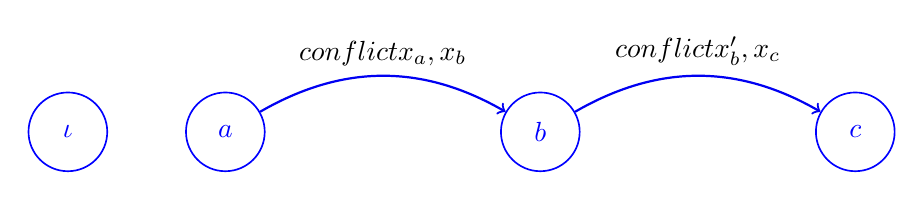
\begin{tikzpicture}[->, semithick]
		\tikzset{
		    tnode/.style= {circle, draw=blue, color=blue, minimum width=1cm},
		    pnew/.style= {below, black!5!blue, thick},
		}
		
		\node[tnode] (s1) at (0, 0) {$\iota$};
		\node[tnode] (s2) at (2, 0) {$a$};
		\node[tnode] (s3) at (6, 0) {$b$};
		\node[tnode] (s4) at (10, 0) {$c$};
		
		\draw
		(s2) edge[pnew, bend left] node[color=black, midway, above] {$\pred{conflict}{x_a, x_b}$} (s3)
		(s3) edge[pnew, bend left] node[color=black, midway, above] {$\pred{conflict}{x_b', x_c}$} (s4);
	\end{tikzpicture}
	\captionof{figure}{A serialization graph which shows conflicting operations between nodes.}
	\label{fig:nodesPath}
\end{center}

In order to better understand this, let's focus on the example provided in Figure \ref{fig:nodesPath} where we labelled the edges of a serialization graph for clarity. We assume that the conflicting operations are instantiated as $x_a = op(a, k), x_b = op(b, k), x_b' = op(b, k')$ and $x_c = op(c, k')$. Now, since it could be the case that $k \neq k'$, there might not exists a conflict between an operation of transaction $a$ and $c$. Still, from Lemma \ref{lem:sg1} we know that transaction $a$ must release the lock on $k$ before $b$ acquires it, and $b$ release the lock on $k'$ before $c$ acquires it. It follows that the $\mathsf{unlock}$ operation of $a$ in $k$ precedes the $\mathsf{lock}$ on $k'$ done by $c$. This intuition is formally verified as part of the following lemma.

\begin{lem}
	\label{lem:sg2}
	\begin{gather*}
	\forall \tau, i, j, n > 0 \ldotp i \rightarrow^n j \in \pred{SG}{\tau} \implies \\
	\exists k, k', \kappa \ldotp op(i, k) \in \tau \land op(j, k') \in \tau \land \tau \vDash \actunlock{i}{k} < \actlock{j}{k'}{\kappa}
	\end{gather*}
	
	{\parindent0pt
	\begin{proof}
	Let's pick an arbitrary trace $\tau \in [\mathsf{Act} \times \mathds{N}]$, such that $\tau = \pred{trace}{h, \emptyset, S, \mathds{P}}$ for some $h \in \mathsf{Storage}$, $\mathds{P} \in \mathsf{Prog}$, $S \in \mathsf{TState}$, $n \in \mathds{Z}$ such that $n > 0$ and transaction identifiers $i, j \in \mathsf{Tid}$. We will prove the lemma by induction on $n$, i.e. the length of the path from node $i$ to node $j$. \\
	\indline
	\textit{Base case}: $n = 1$
	
	We assume that $i \rightarrow^1 j \in \pred{SG}{\tau}$ which, by definition, is equivalent to $i \rightarrow j \in \pred{SG}{\tau}$. From Lemma \ref{lem:sg1} we get that $\exists k, \kappa \ldotp \alpha_i(k) \in \tau \land \alpha_j(k) \in \tau \land \tau \vDash \actunlock{i}{k} < \actlock{j}{k}{\kappa}$ that concludes the proof for this case. \\
	\indline
	\textit{Inductive case}: $n > 1$
	
	\textit{Inductive hypothesis}: Assume the property holds for $n$.
	
	We now want to prove the same property for $n + 1$ so we assume that:
	\begin{gather}
		\label{lem:sg2.1}
		i \rightarrow^{n+1} j \in \pred{SG}{\tau}
	\end{gather}
	From (\ref{lem:sg2.1}) and the definition of $\rightarrow^{n+1}$, we know that for $n$ and for some $t \in \mathsf{Tid}$, the following holds:
	\begin{gather}
		\label{lem:sg2.2}
		i \rightarrow^n t \in \pred{SG}{\tau} \\
		\label{lem:sg2.3}
		\land\ t \rightarrow j \in \pred{SG}{\tau}
	\end{gather}
	From (\ref{lem:sg2.2}) and the inductive hypothesis on $n$ we obtain that, for keys $k_1, k_2 \in \mathsf{Key}$ and lock mode $\kappa_t \in \mathsf{Lock}$, there are two operations $op(i, k_1)$ and $op(t, k_2)$ which are part of $\tau$ and for which the following is true:
	\begin{gather}
		\label{lem:sg2.4}
		\tau \vDash \actunlock{i}{k_1} < \actlock{t}{k_2}{\kappa_t}
	\end{gather}
	From (\ref{lem:sg2.3}) we know that $t \rightarrow j \in \pred{SG}{\tau}$ holds and together with Lemma \ref{lem:sg1} we obtain that, for a storage key $k \in \mathsf{Key}$ and lock mode $\kappa \in \mathsf{Lock}$, there are two conflicting actions $op(t, k)$ and $op(j, k)$ inside $\tau$ such that $\tau \vDash \actunlock{t}{k} < \actlock{j}{k}{\kappa}$. From Lemma \ref{prop:2phase} we obtain that $\tau \vDash \actlock{t}{k_2}{\kappa_t} < \actunlock{t}{k}$ holds, as a consequence of the two-phase rule. Therefore, combined with (\ref{lem:sg2.4}), we then have:
	\begin{gather*}
		\left(
		\begin{array}{c}
			\tau \vDash \actunlock{i}{k_1} < \actlock{t}{k_2}{\kappa_t}
			\land \tau \vDash \actlock{t}{k_2}{\kappa_t} < \actunlock{t}{k} \\
			\land\ \tau \vDash \actunlock{t}{k} < \actlock{j}{k}{\kappa}
		\end{array} \right) \\
		\begin{aligned}
			&\implies \tau \vDash \actunlock{i}{k_1} < \actlock{t}{k_2}{\kappa_t} < \actunlock{t}{k} < \actlock{j}{k}{\kappa} \\
			&\implies \tau \vDash \actunlock{i}{k_1} < \actlock{j}{k}{\kappa}
		\end{aligned}
	\end{gather*}
	We can thus conclude with the required result.
	\end{proof}
	}
\end{lem}

At this point we have formulated and shown all of the necessary ingredients to prove that the serialization graph of any \tpl\ trace does not contain any cycles. As part of the proof, we assume the presence of a generic cycle and using a combination of the previously defined lemmata, show that we arrive at a contradiction.
\begin{thm}
	\label{thm:sgAcyclic}
	(Acyclic serialization graph).
	\[
	\forall \tau, i \ldotp i \in \pred{SG}{\tau} \downarrow_1 \implies \lnot i \rightarrow^* i \in \pred{SG}{\tau}
	\]
	\begin{proof}
	Let's pick an arbitrary trace $\tau \in [\mathsf{Act} \times \mathds{N}]$, such that $\tau = \pred{trace}{h, \emptyset, S, \mathds{P}}$ for some $h \in \mathsf{Storage}$, $\mathds{P} \in \mathsf{Prog}$, $S \in \mathsf{TState}$ and transaction identifier $i \in \mathsf{Tid}$. We assume that $i$ is part of the transaction identifiers in the serialization graph, i.e. $i \in \pred{SG}{\tau} \downarrow_1$. Let's now also assume that the graph contains a cycle on $i$, which means that $\exists n \ldotp i \rightarrow^n i \in \pred{SG}{\tau}$. From Lemma \ref{lem:sg2} we obtain that for some keys $k, k' \in \mathsf{Key}$ and lock mode $\kappa \in \mathsf{Lock}$, $\tau \vDash \actunlock{i}{k} < \actlock{i}{k'}{\kappa}$ which contradicts the two-phase rule defined in Lemma \ref{prop:2phase}. Therefore, by contradiction we conclude that $\lnot i \rightarrow^* i \in \pred{SG}{\tau}$.
	\end{proof}
\end{thm}

For completion, we combine the theorem which was just proven with our results from Section \ref{sec:graphs} in order to formally prove that every \tpl\ trace produced by our operational semantics is serializable.
\begin{thm}
	(Serializability).
	\[
		\forall \tau, h, S, \mathds{P} \ldotp \tau = \pred{trace}{h, \emptyset, S, \mathds{P}} \implies \pred{serializable}{\tau}
	\]
	\begin{proof}
	Let's pick an arbitrary trace $\tau \in [\mathsf{Act} \times \mathds{N}]$ and assume that $\tau = \pred{trace}{h, \emptyset, S, \mathds{P}}$ for program $\mathds{P}$, transactions' stack $S$ and storage $h$. From Theorem \ref{thm:sgAcyclic} we obtain that $\pred{acyclic}{\tau}$ holds and from Theorem \ref{thm:acySer} we know that $\pred{serializable}{\tau}$ holds, which concludes our proof.
	\end{proof}
\end{thm}